\subsection{Offene Fragen}

\subsubsection{ISO 29002-31}
\begin{description}
\item[Abfrage Schnittstelle] Der Standard gibt keine genaue Implementierung vor, erwähnt aber eine Anfrage per E-Mail. Hierfür vermutlich auch die Antwortadresse zwecks automatisierter Antwort ebenfalls per Mail. Wir haben uns bereits auf Web Service geeinigt, da es naheliegt. Kapitel 6 besagt, dass der query\_context entfallen kann falls ein anderer "Hüllen"-Standard wie z.B. EDI genutzt wird. Ich denke das trifft hier zu. 
\item[Conformance class] Welche conformance class sollen wir unterstützen? CC1 - simple query, oder CC2 - parametric query?
\item[XSD] Im Anhand sind XSDs referenziert. Diese wären natürlich für die Implementierung hilfreich.
\item[data\_specification reference] Es wird eine data\_specification\_reference als IRDI mit dem query übermittelt. Womit wird das abgeglichen? Siehe dazu auch weiter unten, die Fragen zu ISO 22745-30.
ISO 29002-31 sagt: 
\begin{quotation}
A query can reference a data specification, which defines the properties for the class of items being queried. The format of the data specification is not specified in this part of ISO/TS 29002. ISO 13584-32 or ISO/TS 22745-30 specify data models and exchange formats that could be used for data specifications.
\end{quotation}
\end{description}


\subsubsection{ISO 22745-30}
\begin{description}
\item[IG Anwendung] Da der Identification Guide beschreibt, welche Daten überhaupt sinnvoll sind, stellt sich die Frage wohin diese Abfrage gestellt wird. Verstanden habe ich es so, dass der Kunde jeweils selbst diese Daten pflegt. Die ISO 22745-30 sagt dazu \begin{quote}
Most data recipients require data describing items belonging to more than one class. An identification guide group is a collection of identification guides that, together, describe the data recipient's requirements for describing items belonging to more than one class.
\end{quote} Es ist offensichtlich so, dass der Datenempfänger definiert welche Datenqualität er benötigt und welche nicht. 
Folglich verstehe ich das so, dass der IG nicht gleichzusetzen mit einem "select" in SQL ist, sondern beschreibt welche Properties einer Class abgefragt werden sollten damit überhaupt sinnvoll damit umgegangen werden kann, denn das Dictionary wird offensichtlich eine große Menge an Properties beinhalten die für bestimmte Kunden für dessen Anwendung nicht sinnvoll sind. Stellt sich die Frage, ob ich den IG umsetzen soll? Der "select"-Teil eines Queries kann bereits mit 29002-31 gestellt werden, nur weiß der Kunde nicht welche Properties er für einen bestimmten selbstdefinierten Zweck benötigt. Das muss er vorab definieren. Aber ein XML aus 22745-30 welche das beschreibt wird nicht an den Datenbereitsteller geschickt. 
EIn Identification Guide wird auch verglichen mit einem Formular, welches definiert welche Formularfelder enthalten sein sollen. Man könnte somit das Abfrageformular hieraus generieren. Stellt sich die Frage ob dies so dynamisch sinnvoll ist. 
\item[IG Abfrage] Soll der IG umgesetzt werden, ist mir nicht klar, wie das passieren soll. Beschrieben wird in diversen Präsentationen aus dem Internet \(z.B. ECCMA^\_ISO\_8000\_certification.pdf\), dass der IG sich auf Kundenseite befindet. 
Wie erfolgt die Abfrage dann? Auf welcher Datenbasis? Wohin wird solch eine Abfrage geschickt bzw woher wird die Spezifikation der Datenqualität geholt? Siehe Abbildung \ref{fig:ig_query_response}

\item[XSD] Im Anhand sind XSDs referenziert. Diese wären natürlich für die Implementierung hilfreich.
\end{description}


\begin{figure}[htbp]
	\centering
		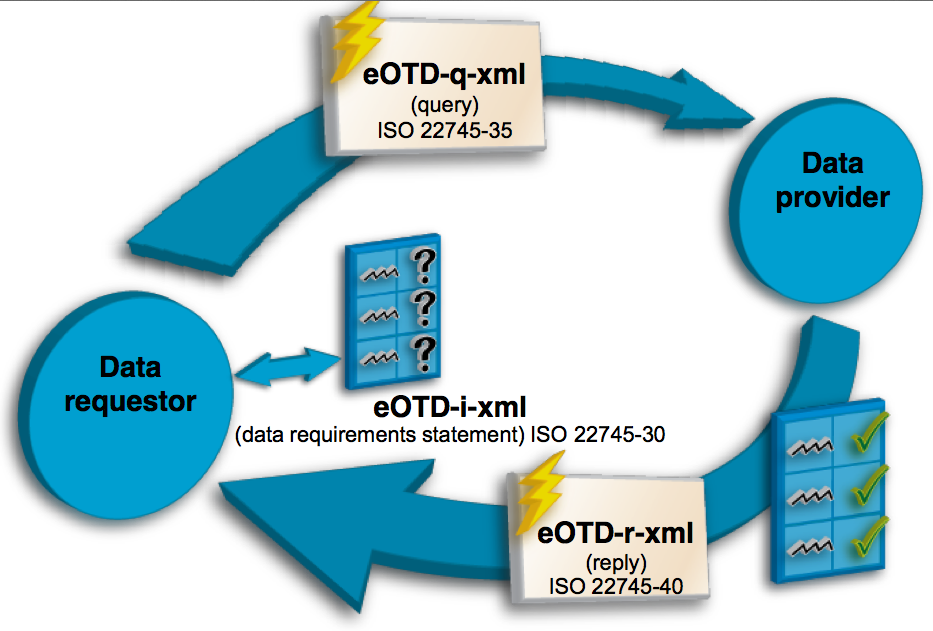
\includegraphics[width=0.8\textwidth]{images/ig_query_response.png}
	\caption{Ablauf eines queries}
	\label{fig:ig_query_response}
\end{figure}
